\documentclass[12pt, a4paper]{report}
\usepackage{graphicx, listings, framed, mdframed, float}
\usepackage{appendix, pdfpages, setspace, color, hyperref}
\usepackage{tocloft}                    % This squashes the Table of Contents a bit
\hypersetup{colorlinks=true}            % To avoid the borders around hyperlinks
\hypersetup{colorlinks, citecolor=black, filecolor=black, linkcolor=black, urlcolor=black}
\definecolor{MyLightYellow}{cmyk}{0,0.,0.2,0} % Used for program listings 
\definecolor{shadecolor}{cmyk}{0,0.2,0,0} % Used for snugshade listings 
\usepackage[top=3cm, bottom=3cm]{geometry}% page margins
\usepackage{rotating}   
\setlength{\parskip}{10pt}                % sets spacing between paragraphs
\interfootnotelinepenalty=500             % this prevents footnotes breaking across pages
\renewcommand\bibname{References}         % to change Bibliography to References
\renewcommand\lstlistlistingname{List of Code Listings}
\newcommand{\HRule}{\rule{\linewidth}{0.75mm}} % needed on title page

\begin{document}

\begin{titlepage}   % Standard template for title page. Please don't change layout.
\begin{center}
% Upper part of the page

\includegraphics[width=0.4\textwidth]{BigCrest}\\ \vspace{15 mm}   
\textsc{\Large Year 2 Project}\\ \vspace{15 mm}
\doublespace
\HRule \\ \vspace{8 mm}
{\huge \bfseries Frequency Downconverter}       % <<<< Put your title here
\\\vspace{4 mm}
\HRule \\ \vspace{25 mm}

Yimian \textsc{Liu} (ID 201448055)      \\        % <<<< Your names
Boyao \textsc{Yang} (ID 201448734)      \\        % <<<< Your names
Weizhou \textsc{Wen} (ID 201448566)      \\        % <<<< Your names
Yidi \textsc{Song} (ID 201448330)      \\        % <<<< Your names
Group 61                                 \\        % <<<< Your group number

\vspace{15mm}
\emph{Supervised by } Dr Christos \textsc{Zachariades}     % <<<< Your supervisor

\vfill             % Bottom of the page
{\large \today}    % today's date
\end{center} 
\end{titlepage}


\begin{abstract}
Frequency Downconverter (FDC) is used in signal processing equipment to converter ratio frequency signal to low frequency signal. The low frequency signal is more convenient for signal processing \cite{ref:zhang}. In the project, a basic circuit of FDC was designed by student firstly. Then, a Printed Circuit Boards (PCB) of FDC was designed with software Eagle CAD and Altium Designer (AD). Then, the basic PCB was manufactured by Electrical and Electronic Engineer Department with the diagram. The test of products is also in the schedule initially. However, the whole products have not been finished in the end. In the project, students learnt how to understand the datasheet of components. Then, students learnt how to design circuit and PCB with software. The study of software for communication and documentation are also helpful, including Git and \LaTeX. The knowledge and experience in the project are meaningful in the future career of students.
\end{abstract}

\newpage

\rule{0mm}{30mm}

\centerline{\textbf{Declaration}}

\fbox{\parbox{0.92\textwidth}{I confirm that I have read and understood the University’s definitions of plagiarism and collusion from the Code of Practice on Assessment. I confirm that I have neither committed plagiarism in the completion of this work nor have I colluded with any other party in the preparation and production of this work. The work presented here is my own and in my own words except where I have clearly indicated and acknowledged that I have quoted or used figures from published or unpublished sources (including the web). I understand the consequences of engaging in plagiarism and collusion as described in the Code of Practice on Assessment (Appendix L).}}



\newpage \tableofcontents
\newpage \listoffigures
\newpage \listoftables 

\newpage \onehalfspace



\chapter{Introduction}

\section{Problem and Motivation}
In the signal device, the electrical components which can work for radio frequency signal are expensive and scarce. In the project, the group members aimed to design a Frequency Downconverter (FDC). The product device can convert a high-frequency ratio signal to low frequency signal, and it is used in signal process equipment. Then, the low frequency signal can be amplified by cheap and widely used components. Meanwhile, the information stored in the signal is preserved. As a result, it is not necessary to use expensive components for high frequency in the whole signal equipment, and the cost of signal equipment is likely to be reduced. 

\section{Literature Review}

There are basically three solutions to get a frequency converter. The first method is to utilize the technology of Field Programmable Gate Arrays (FPGA) to design a digital down converter \cite{yang}. The second way is to design a Printed Circuit Boards (PCB) working with analog components and Integrated Circuit (IC) such as mixers and amplifiers. In addition, a FDC IC can also be designed with Complementary Metal-Oxide-Semiconductor (CMOS) technology \cite{cmos}.

\newpage

\begin{figure}[htbp]     \begin{centering}
    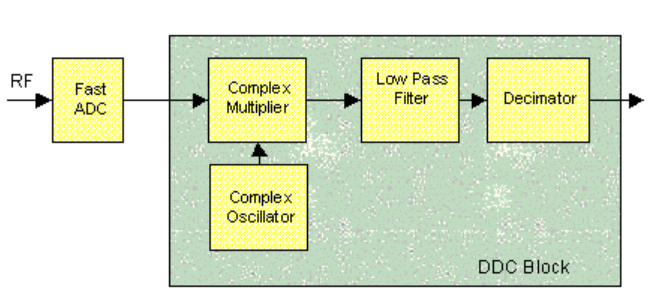
\includegraphics[width=0.5\textwidth]{img/ddcb.png}
    \caption{\label{Fig:ddcb}Digital Frequency Down Converter Model \cite{hunteng.co.uk}}
    \end{centering}
\end{figure}

A Digital Down Converter (DDC) working after an Analog-Digital Converter (ADC) which functions to convert the analog Radio Frequency (RF) signal to digital format consists of a complex multiplier, a Low Pass Filter (LPF) and a decimator \cite{hunteng.co.uk}, as it shown in Figure \ref{Fig:ddcb}. In theory, a FPGA FDC consists of a digital oscillator, a digital multiplier, and digital filters \cite{yang}. The key challenge of this method is the design of FPGA models including NCO (generating cosine signal), CIC Filter (sampling), HB Filter (second sampling), FIR Filter (eliminating noise) \cite{xu}.


\begin{figure}[htbp]     \begin{centering}
    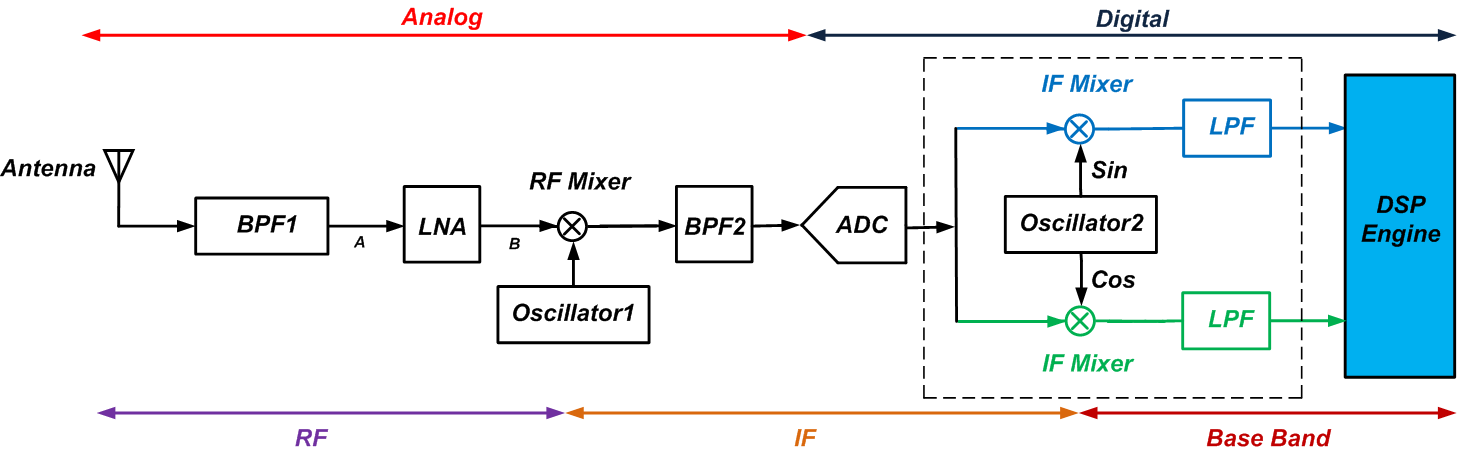
\includegraphics[width=1.0\textwidth]{img/ddc.png}
    \caption{\label{Fig:ddc}Analog Frequency Down Converter Model \cite{ref:ddc}}
    \end{centering}
\end{figure}

Figure \ref{Fig:ddc} proposed by Steve Arar \cite{ref:ddc} provides a viewpoint of how an analog FDC is designed. The RF signal is collected with an antenna and is transmitted through a Band Pass Filter (BPF) and a high-quality amplifier (LNA). A RF mixer accepts the RF signal and a Local Oscillator (LO) signal to give out the result of multiplication. The resulting signal then goes through the second Band Pass Filter and is then converted into digital format through an ADC.

Different from the analog method, instead of using discrete components, the CMOS method uses semiconductor materials and related technic to build the circuit. This method can achieve the function of FDC in considerable small scale and is suitable to deal with relatively high frequency such as 2.4GHz \cite{cmos}, however, the difficulty and cost of R&D can not be underrated. 

Comparing with the FPGA method, the analog method seems can not easily include a oscillator and may need an extra signal generator for generating LO signal. Moreover, the size of the circuit of analog method may not be designed as small as the CMOS method. Nevertheless, it has low development cost and may be more friendly to be chosen as the first shoot for freshmen.

As for the craft of PCB design, firstly, Electromagnetic compatibility (EMC) problems exist in the overall layout of PCBs, wiring, distribution of vias, and ground design \cite{ref:l0}. Therefore, the EMC problem should be considered in the whole process of PCB design, as well as the EMC could be simulated by software. The Electromagnetic Interference (EMI) in PCB may come from parasitic coupling between adjacent circuits and field conversion between internal components, while external problems are divided into radiation and sensitivity \cite{ref:l0}. Especially in RF circuit, it is easy to produce a coupling effect in the actual work. In addition, cross-talk is one of the main obstacles for high-speed circuits to achieve their initial signal. Generally, far-end cross-talk can be mitigated by transitioning the length of high-frequency traces, increasing the spacing between traces and inserting current strength \cite{ref:l1}. In the high frequency circuit, the impedance is reactive including capacitive and inductive, which is substantially higher. Moreover, PCB stack generation and characterization planning should be performed in the initial stage of PCB design \cite{ref:l2}.

\section{Specific Objectives}
On the basis of literature review, an analog FDC was decided to be designed, manufactured and tested. To reach the objective, the group members need to finish following tasks:
\begin{enumerate}
\item Design a basic electric circuit for the device and decide the components purchase lists.
\item Use PCB design software Altium Designer (AD) and Eagle CAD to design the printed circuit.
\item Use Surface Mount technology to solder other components to the printed circuit.
\item Test the products and record the spectrum of the output signal. 
\end{enumerate}

\section{Road Map}

In the report, the basic material (software and hardware) and design methods are introduced. Then, the result of the projects is assessed and analyzed. Next, the technical details, progress and mistakes are discussed. Finally, students summarize the project of FDC.




\chapter{Materials and Methods}


\section{Materials}

\subsection{Software Tools}


\begin{enumerate}

\item \textbf{Altium Designer v20.0.1} 

Altium Designer is an electronic product development system which is used for Electronic Design Automation (EDA) including Schematic drawing, production of Printed PCB files and circuit simulation. This software was used to design most parts of the schematic and PCB designing works.

\item \textbf{Autodesk Eagle v9.5.1}

EAGLE is also an EDA software which enables PCB designers to seamlessly connect schematic diagrams, component placement, PCB routing, and comprehensive library content. This software was used at the last stage of the project to meet the requirement of department workshop.

\item \textbf{Advanced Design System 2020}

Advanced Design System (ADS) software gives accurate and functional simulation for high-frequency RF circuits. This software was used to verify the explore the frequency response of various types of filters and verify the effect of the designed LPF.

\item \textbf{Git 2.26.0}

Git is a distributed version control system which is designed by the father of Linux to promote team project management. This tool was mainly utilized to trace changes and support the rolling development between schematic design and PCB design.

\end{enumerate}



\subsection{Equipment List}

\begin{enumerate}

\item \textbf{Oscilloscope}: TBS 1052 B-EDU
\item \textbf{DC Power Supply}: TENMA 72-8695A
\item \textbf{Signal Generator}: Digimess FG303 (or others)
\item \textbf{Digital Multimeter}: TENMA 72-1016
\item \textbf{Spectrum Analyzer}: ROHDE&SCHWARZ FSC3

\end{enumerate}


\subsection{Components Suppliers}
\begin{enumerate} \addtolength{\itemsep}{-0.5\baselineskip}
    \item Onecall (http://onecall.farnell.com)
    \item RS (http://uk.rs-online.com)
\end{enumerate}

\section{Circuit Design}

In this part, an analog FDC circuit is expected to be designed with a 300MHz-3GHz RF input and a 30MHz-300MHz Intermediate Frequency (IF) output. 


\begin{figure}[htbp]     \begin{centering}
    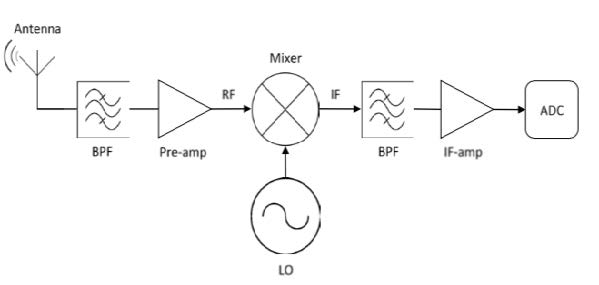
\includegraphics[width=0.8\textwidth]{img/model.jpg}
    \caption{\label{Fig:model}General Analog FDC Model}
    \end{centering}
\end{figure}


As it shown in Figure \ref{Fig:model}, a typical FDC consists of three parts: a mixer, filters and amplifiers. The mixer accepts two signal, the RF signal which is collected through an antenna and has been processed through a BPF and a high-quality amplifier (LNA), and the LO signal which needs to be provided externally. 


\begin{equation}
S_{IF} = cos(\omega_{RF}t) cos(\omega_{LO}t)
\label{eq:mixer}
\end{equation}

Equation \ref{eq:mixer} shows the output of the IF signal from the mixer, under the condition that the RF and LO signal are ideal cosine functions towards time with angular velocity of $\omega_{RF}$ and $\omega_{LO}$. The mixer exports the multiplication of these two signal in time domain.

\begin{equation}
S_{IF} = [cos(\omega_{RF}t+\omega_{LO}t)+cos(\omega_{RF}t-\omega_{LO}t)]/2
\label{eq:mixer2}
\end{equation}

After applying the product and difference formula, Equation \ref{eq:mixer2} can be inducted. As the angular velocity can be presented by frequency as $\frac{f}{2\pi}$, the result in frequency domain then can be calculated.

\begin{equation}
F_{IF} = \frac{F_{RF}+F_{LO}}{2}+\frac{F_{RF}-F_{LO}}{2}
\label{eq:mixer3}
\end{equation}

Equation \ref{eq:mixer3} indicates the relationship among the frequency of RF, LO and IF signal. It can be inferred that the resulting IF signal is a combination of two signal, the $F_{RF}+F_{LO}$ signal and the $F_{RF}-F_{LO}$ signal.


\begin{figure}[htbp]     \begin{centering}
    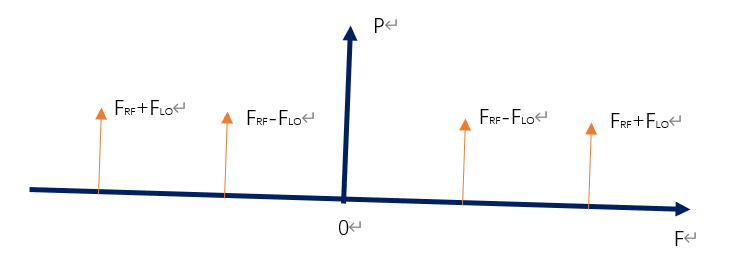
\includegraphics[width=0.8\textwidth]{img/ff.png}
    \caption{\label{Fig:ff}IF Diagram in Frequency Domain}
    \end{centering}
\end{figure}

Figure \ref{Fig:ff} displays the IF signal in frequency domain. As both of these two signal contain all the information of the RF signal, it can be indicated that if a LPF with a cut-off frequency between $F_{RF}-F_{LO}$ and $F_{RF}+F_{LO}$, a signal at $F_{RF}-F_{LO}$ frequency can be obtain with all the information remaining.

\newpage

\begin{figure}[htbp]     \begin{centering}
    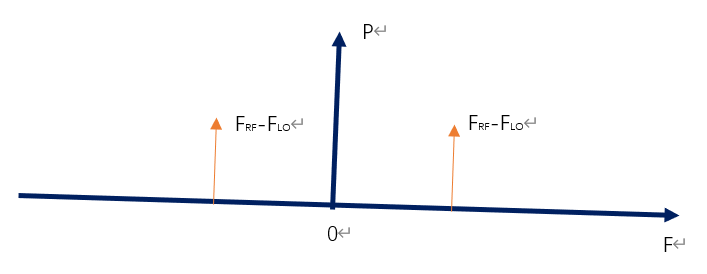
\includegraphics[width=0.8\textwidth]{img/fff.png}
    \caption{\label{Fig:fff}IF (after LPF) Diagram in Frequency Domain}
    \end{centering}
\end{figure}

Figure \ref{Fig:fff} shows the frequency domain situation of IF signal after the implement of LPF. This signal can then be sampled by ADC and be processed through other digital circuits.

As all complex signal can be decomposed into sine and cosine expressions with Fourier Series \cite{book}, the derived conclusion in the condition that RF and LO are two simple cosine waves can be generalized to all complex cases. 

Since the purpose of this project is to learn the basic design knowledge, the designing is expected to be as simple as possible to avoid mistakes. Therefore, only necessary parts of a mixer and a LPF was required to be presented, while the mixer is used to mix the RF and LO signal and the LPF was used to block the high frequency useless signal to get the final low frequency signal.

\subsection{IC Selection}

The first step to design the circuit was to clarify the functions and roles of the most important part, which was the mixer in this case. After search for available mixer on the supplier's websites, it was found that most of the mixers was manufactured as IC. Therefore, a mixer IC was need to be selected. As the objective of this project was to convert the signal in frequency 300MHz-3GHz (VHF) to 30MHz-300MHz (UVF), this IC needed to accept the signal working at VHF and can output signal working in UVF range. Besides, this IC was also expected to have a lower loss (less noise) and high insulation among different ports.

The general parameters that describe frequency mixer are listed in the following list.

\newpage

\begin{enumerate} \addtolength{\itemsep}{-0.5\baselineskip}
    \item \textbf{Noise Figure:} The parameters that reflects the noise generated mainly by inner circuit.
    \item \textbf{Loss:} The power loss of the signal input.
    \item \textbf{Frequency Range:} The frequency range of input RF signal.
    \item \textbf{Insulation:} The parameter that describe the insulation between different input ports.
\end{enumerate}


In addition, it was expected that the IC could accept a wide range of frequency so that the design can be flexibly changed in the following design stage. It was also considered concerning the support from the IC datasheet and the scale of its communities (products using this IC). Moreover, as the IC is working at very high frequency, its size may be smaller than common IC. It should also be considered regarding whether the university can manufacture the circuit with this IC. From the perspective of cost, the price of the IC should also be considered. However, as the aim of this project is study, this point was not as important as others.

From the above paragraphs, it can be concluded that an idea mixer IC should have the following characters.

\begin{enumerate} \addtolength{\itemsep}{-0.5\baselineskip}
    \item \textbf{Flexibility:} Can accept a large range of input and output frequency.
    \item \textbf{Support:} The availability of official and community support.
    \item \textbf{Quality: } Less loss and less noise with high insulation.
    \item \textbf{Difficulty:} The difficulty of manufacturing (the size of the IC). 
    \item \textbf{Cost:} The price of the IC.
\end{enumerate}

Finally, LT5512\cite{ref:LT5512} from Linear Technology was selected because of its wide frequency range supported and excepted performance, while few other similar IC can be found on the university supplier's websites.

According to LT5512 datasheet \cite{ref:LT5512}, this mixer is active and may need an extra 5V DC power supply. Comparing with other passive mixers which do not require an external power source, LT5512 have a significantly low loss rate and even have a 1 dB gain due to its inner buffer design. Besides, LT5512 has a high LO-RF isolation which can reduce the possibility of disturbance among ports. Another advantage of LT5512 is that it can work at a wide RF and IF range from 10MHz to 3GHz, while it has a relatively low noise with a SSB Noise Figure of 11dB at 900MHz.

Nevertheless, the disadvantage of LT5512 is that it is packaged in 4mm x 4mm QFN Package, which make it quite difficult to be designed and manufactured. The other shortage of LT5512 is that few products using this IC can be found on internet and the official support is poor as the old team from Linear Technology had been reformed into as new company called Analog Devices.

\subsection{Impedance Matching}

After the selection of IC, the impedance of the circuit should be specially designed to match other modules. The reason for this is that the FDC circuit we were designing was expected to be a standard module that can interact with other standard modules. Therefore, the input and output of the circuit should be designed to be 50 ohms to decrease the loss and disturbance of signal.

There are several methods to do the impedance matching for the circuit. Firstly, the datasheet recommends several situations with the detailed value of capacitors and inductors for the impedance matching for IF, LO and RF part at different frequency. To avoid mistakes, these circuits were directly used to design the impedance matching in FDC case. Then, if a datasheet recommended method does not exist, other tools such as online computing tools, Smith Chart and directly computing via Thevenin theorem can be utilized.

\subsubsection{1.9GHz-170MHz Version}

At the beginning of the project, the working frequency of the circuit was set to be 1900MHz to 170MHz to meet the requirement. The reason for choosing this frequency was that there were cases from datasheet and official materials can be referred. The circuit can be designed with only a few changes which was able to avoid a lot of mistakes to make the circuit work. Besides, designing a circuit working at such frequency may require extra RF knowledge such as differential line which we may benefit from the learning process when trying to understand the official demo.




\begin{figure}[htbp]     \begin{centering}
    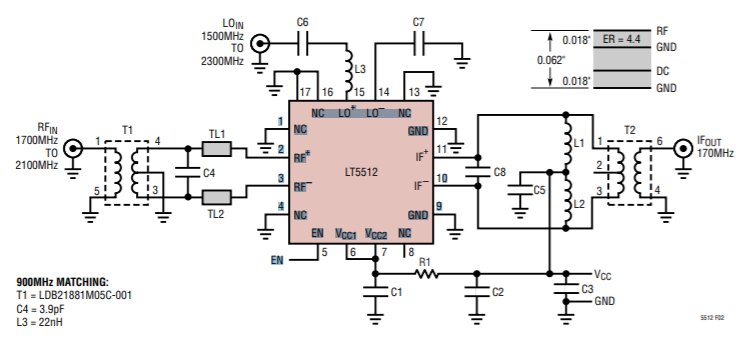
\includegraphics[width=0.8\textwidth]{img/d1.png}
    \caption{\label{Fig:d1}LT5512 Datasheet Demo Circuit at 1900MHz RF (taken from~\cite{ref:LT5512_old})}
    \end{centering}
    
\end{figure}

\newpage

From Figure \ref{Fig:d1}, a demo circuit working at 1.9GHz-170MHz was presented. This circuit can be divided into four part: RF part (left), IF part (right), LO part (upper) and VCC part (lower). As the RF part working at 1.9GHz need a lot special knowledge when designing, we directly use its design.



\begin{figure}[htbp]     \begin{centering}
    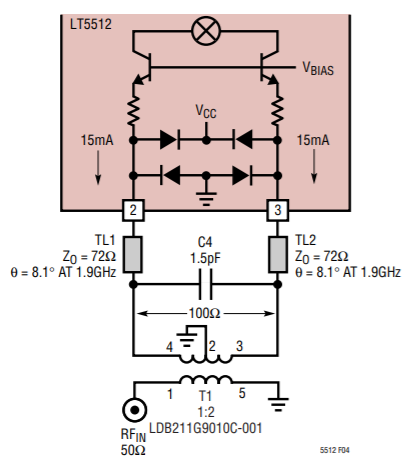
\includegraphics[width=0.5\textwidth]{img/d1_rf.png}
    \caption{\label{Fig:d1_rf}1900MHz RF Circuit (taken from~\cite{ref:LT5512_old})}
    \end{centering}
    
\end{figure}

For the RF part, after a 1:2 Balun transformer, the equivalent impedance is 100 ohms, as it shown in Figure \ref{Fig:d1_rf}. The equivalent impedance of the IC can be checked to be $20.6+j22.8$ ohms. Then, the value of $C_{4}$ and $T_{L}$ can be calculated using Thevenin theorem. 

\begin{equation}
100\ohm=-\frac{j}{2\pifC_{4}} /\kern -0.8em / (Z_{IC}+Z_{line})
\label{eq:d1_rf}
\end{equation}

From Equation \ref{eq:d1_rf}, the value of $C_{4}$ and the line impedance can be computed. As the frequency 1.9GHz is considerably high and the signal can easily escape from the wire, differential line was designed to make the disturbance from the wire can counteract each other and eliminate the overall disturbance.

From the LO part of Figure \ref{Fig:d1}, it can be shown that the capacitors $C_{6}$ and $C_{7}$ were used to block the DC part of input LO signal. While the $L_{3}$ inductor was added here to remove the very high frequency noise basing on experience.

In the lower part of Figure \ref{Fig:d1}, a set of capacitors with different values were added to eliminate noise at different frequency. This measure was also conducted through experience. 

For the IF part in Figure \ref{Fig:d1}, a capacitor in parallel and two inductors was used to match the impedance to 400 ohms and enhance the insulation of the IC. After that, a 8:1 Balun transformer was implemented to decrease the impedance to 50 ohms.


\subsubsection{610MHz-80MHz Version}

\begin{figure}[htbp]     \begin{centering}
    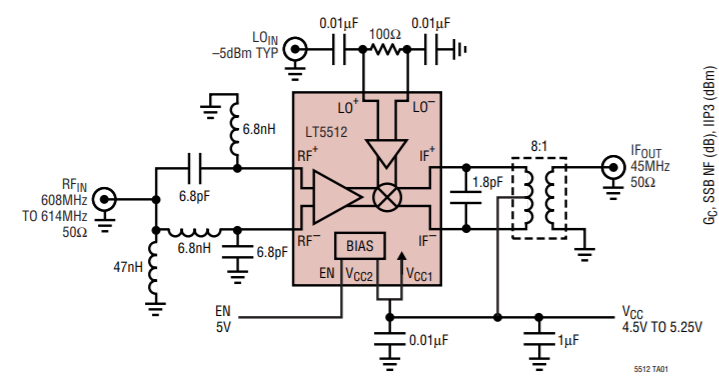
\includegraphics[width=0.8\textwidth]{img/d0.png}
    \caption{\label{Fig:d0}LT5512 Datasheet Demo Circuit at 610MHz RF (taken from~\cite{ref:LT5512})}
    \end{centering}
    
\end{figure}


Considering the difficulty of design and components purchase, the working frequency of FDC circuit was eventually set at 610MHz RF input and 80MHz IF output. Figure \ref{Fig:d0} displays a demo circuit working at 610MHz RF with 50 ohms input impedance. Thus, the RF part of this demo can be used in our circuit for impedance matching. Besides, as the IF frequency is 45MHz which is like the 80MHz in FDC case, the LO frequency is similar and the LO part of the circuit was referred. Moreover, the power supply line was also designed like this demo.

However, for the IF case, the circuit on the datasheet cannot be used since the 1:8 Balun transformer on the recommended circuit cannot be found in UK market. This may mean that, the IF part needs to be designed by other methods.

As the mixer is a non-linear component and it can perform different impedance at different frequency. Thanks to the LT5512 datasheet \cite{ref:LT5512}, the equivalent impedance from different port at different frequency was presented. Basing on this information, the values of capacitors and inductors can be calculated.

\begin{figure}[htbp]     \begin{centering}
    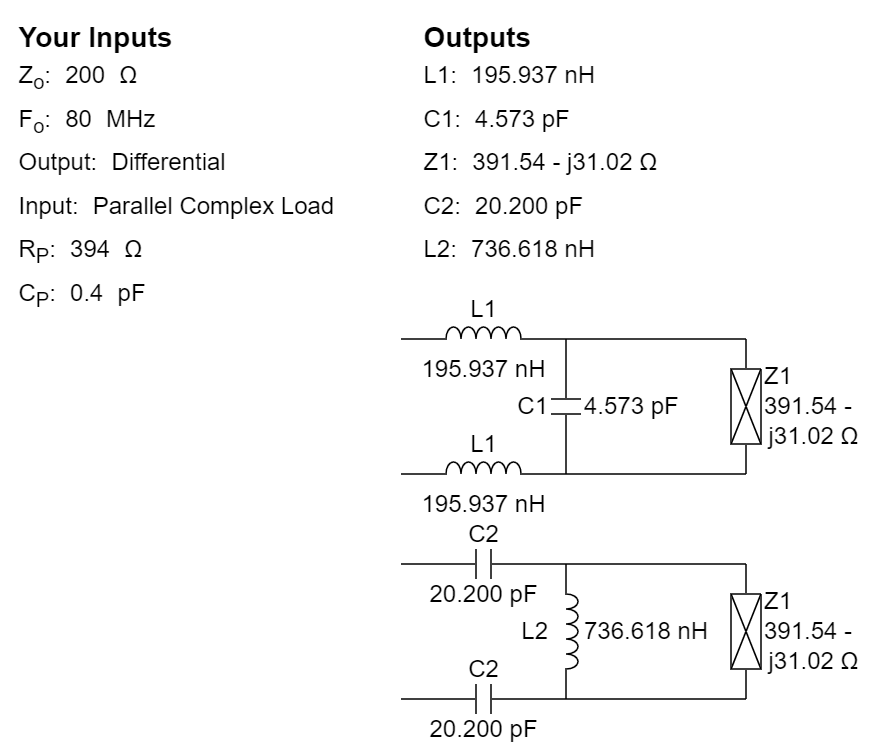
\includegraphics[width=0.5\textwidth]{img/d0_if.png}
    \caption{\label{Fig:d0_if}Impedance Matching of 80MHz IF (calculated from~\cite{ref:rf_im})}
    \end{centering}
    
\end{figure}

Since only a 1:4 Balun can be found in UK market, the output of the RF differential line can only be no more than 200 ohms. In this case, online tools \cite{ref:rf_im} from Analog Device was used and the result was displayed in Figure \ref{Fig:d0_if}. As a Low Pass Filter character is also required in our case, the first schematic in Figure \ref{Fig:d0_if} was used. Besides, according to LT5512 Datasheet\cite{ref:LT5512}, the value of the parallel capacitor should be larger to enhance the insulation of IC. Finally, for the convenience of purchase, the two inductors were set to be 220nH and the capacitor was set to be 5.6pF.

\subsection{Filter Design and Simulation}

There are different kinds of filter such as Butterworth, Chebyshev, Elliptic and Bessel. Comparing with other types, Butterworth filter have the flattest bandwidth, which have few ripples on it, however, the edge of the bandwidth does not decrease quickly. Chebyshev have a relatively quicker decrease at the edge but with more ripple on the bandwidth. The Elliptic change sharply at the edge but with less flat bandwidth. Bessel has the most considerable group delay, which is suitable for audio processing. In FDC case, little ripple can significantly change the signal but it not necessary for the edge to decrease quickly, where Butterworth seems to be more suitable.


\begin{figure}[htbp]     \begin{centering}
    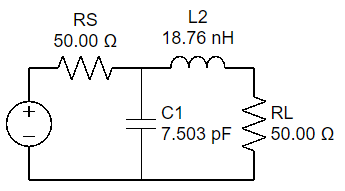
\includegraphics[width=0.5\textwidth]{img/sim0.png}
    \caption{\label{Fig:sim0}Butterworth LPF cutoff at 600MHz (designed from~\cite{ref:rf_tools})}
    \end{centering}
    
\end{figure}


RF Filters online designing tools\cite{ref:rf_tools} was utilized to show the ideal 2 order circuit for 50 ohms to block noise that more than 600MHz. As it shown in Figure \ref{Fig:sim0}, the low pass filter cutoff at frequency 600MHz has a inductor of 18.76nH and a capacitor of 7.5pF. This result was like the impedance result from the last section.

In the 610MHz-80MHz Version, the IF part also need a LPF to block the high frequency noise. In the last subsection, it had already been considered when selecting the method of impedance matching. After that, simulation using Advanced Design System (ADS) was conducted to present the ideal frequency response of the IF circuit.

\begin{figure}[htbp]     \begin{centering}
    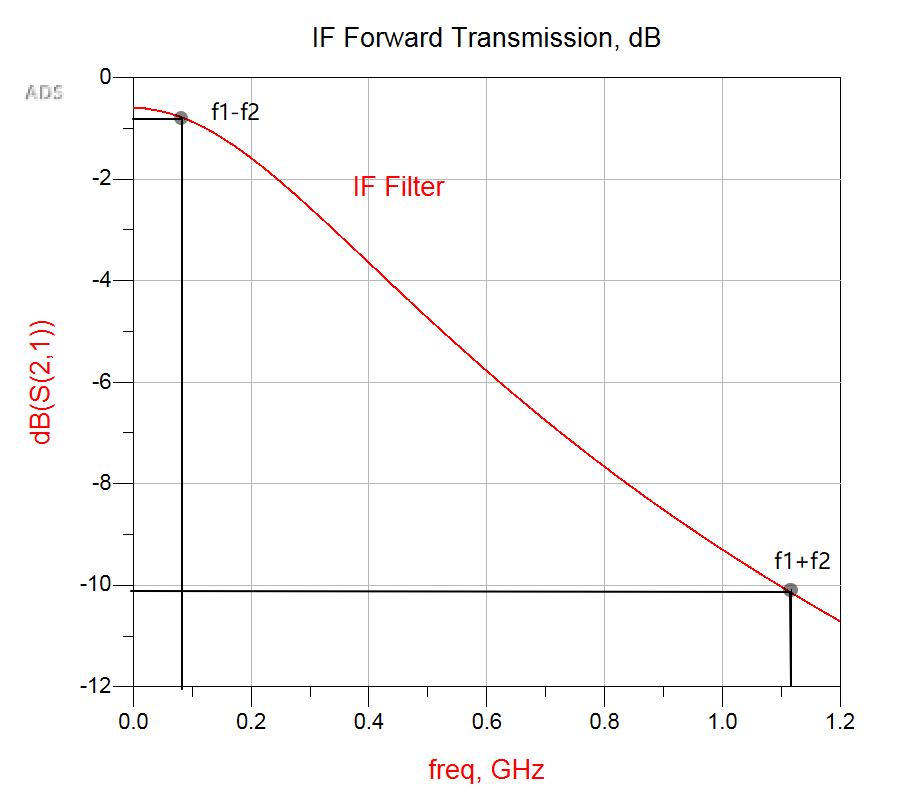
\includegraphics[width=0.5\textwidth]{img/sim1.png}
    \caption{\label{Fig:sim1}Frequency Response of 80MHz IF Circuit (using ADS)}
    \end{centering}
    
\end{figure}

Figure \ref{Fig:sim1} shows the result of ADS simulation of 80MHz IF Circuit. It can be indicated that the output signal working at frequency $f_{1}-f_{2}$ will be weaken about 1dB while the noise working at frequency $f_{1}+f_{2}$ will be decreased by more than 10 dB. This result seems to point that the design of the low pass filter will work as expected.


\subsection{Component Selection and Purchase}

After the design of the schematic, the components list can be proposed. Every time add a new component when designing the circuit, the first thing we do is to check the supplier's websites. The components that have both official library and footprint are preferred. However, when the schematic was finished, the components also need to be checked in case if it sold out during the designing period. Besides, every datasheet of the components need to be checked carefully. Because we are learning the design skills through this project, we may not realize the importance of some parameters such as the work frequency and we may also not understand correctly about some parameters such as the Balun ratio at the first time we select them. Therefore, final check of the datasheets are necessary for the success of this project.

When do the purchase, one point which may also need to be careful is that, some components on the supplier's websites may not use the same name that we call them. For example, we use the words male and female to distinguish the Bayonet Nut Connector (BNC) components. However, they were called as plug and jack on the website.

Another thing that need to be noticed is about the package. As this project is dealing with Surface Mount Device (SMD) components, some of the goods on the website may show in stoke but can only be sold with rolls. The package type of these components should also be considered concerning whether the university could deal with them.

After the components list was confirmed, it can be submitted to the lab after the signature of Academic Advisor.


\section{Components Library}

Before the PCB design, the component library of the schematic and the PCB must be created. In order to ensure the accuracy of component package specifications including footprint, most packages in the PCB component library were imported from the official website of suppliers. The search engine called Altium Octo-part was used to help electronics designers find the suitable components for PCB designs, as well as the relevant data of components could be provided to improve the accuracy and the convenience of the design. Other components which cannot be found from the official website were import from GitHub. There are large number of packages of different types of components has been created on the GitHub. Once the component had been successfully imported, the package specifications and 3D model can be found in the PCB library, and the footprint can be directly placed into the PCB design file. The PCB library contains an integrated circuit which is a Downconverter Mixer, a Balun transformer, the resistance, capacitance and inductance in peripheral circuits and three BNC connectors. After the libraries had been created, the packages data were collated the packages data with the datasheet of every single component.

\section{PCB Structure Design}

Due to the small number of PCB design components and the complexity of the circuit, single-layer design was selected to simplify design and production, and this design uses the double-sided printed board. The line can extend to another side through the via, so one of the most important feature of the single-layer double-sided board is that it has via. A via is a small hole filled or coated with metal on the PCB which can be connected to the wires on both sides of the board.

\section{PCB Layout}

Because the RF circuit is a distributed parameter circuit, it is easy to produce a coupling effect in the actual work of the circuit. Therefore, in the actual PCB design, it will be found that the interference radiation in the circuit is difficult to control. For example, problems such as mutual interference between digital circuits and analogue circuits, noise interference from power supplies, and interference caused by unreasonable ground lines. 

\begin{figure}[htbp]     \begin{centering}
    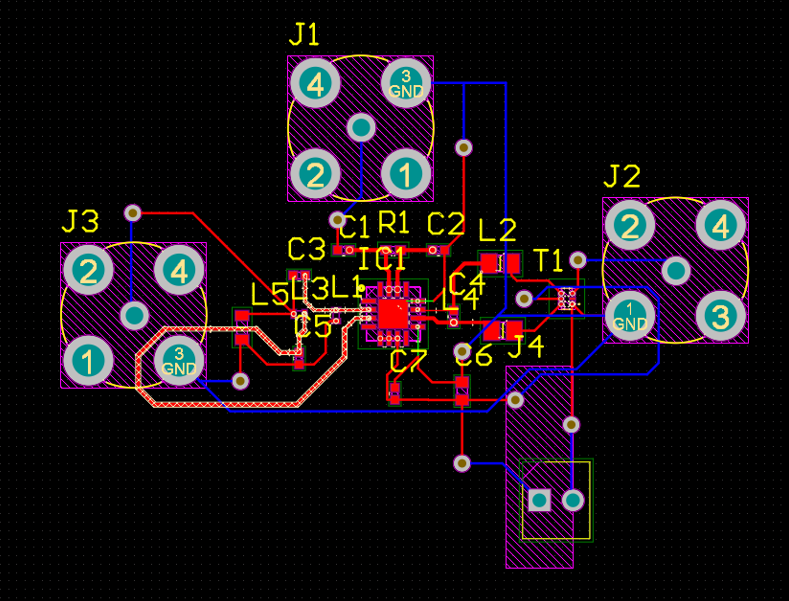
\includegraphics[width=0.5\textwidth]{img/e0.png}
    \caption{\label{Fig:e0}PCB layout and Routing}
    \end{centering}
   
\end{figure}

Therefore, the PCB layout mainly refer to the datasheet of the integrated circuit and the circuit layout of the schematic. As it shown in Figure \ref{Fig:e0}, the IC was placed in the central position, and the Balun transformer was placed on the left of the IC. Resistors, inductors and capacitors in peripheral circuits basically adopted a flat layout and a symmetrical layout. Four interfaces are placed on the periphery of the circuit. The overall layout is basically the same as the relative positions of the components in the schematic.



\section{PCB Routing}

Once the basic placement has been completed, the next stage of the PCB design is to route the connections between all the components. First, the board size and number of wiring layers should be determined. The PCB routing process in this project was conducted on both top layer and bottom layer. Moreover, the PCB routing process should be completed with proper design rules. Different types of signal traces have specific routing requirements. Therefore, it is necessary to classify and set rules for signal cables with special requirements. The first routing uses the software's auto-routing function, then repair the wires according to the specific components and circuits, and all the ground lines were connected to bottom layer through the via.

The overall requirements for wiring are RF signal traces are short and straight, reducing abrupt changes in the line, fewer holes are punched during routing, and they do not intersect with other signal lines. Ground via should be added around the RF signal lines as much as possible.

After designing the routing, pads, and via, a Design Rule Check (DRC) should be performed. In the inspection results, the differences between the designed graph and the defined rules are listed in detail, and the networks that do not meet the requirements can be found.


\section{Copper Plating}

The main purpose of copper plating is to improve the anti-interference ability of the circuit. At the same time, it has great benefits for PCB heat dissipation and PCB strength. Copper grounding can also serve as a shield.

In terms of the design rule setting, the distance between copper and wire or via should be set. In high-frequency circuits, a ground (GND) copper isolation shield is required. Therefore, a large area of copper is applied on the bottom layer to connect all ground wires. For the top layer, the circuit requires strict impedance control, and copper plating is likely to affect impedance control due to distributed capacitance. The wiring density around the integrated circuit is high, and the excessive copper separation may affect grounding. Therefore, large area copper plating is not applicable on the top layer, and grid copper can be used. However, there is no copper plating operation on the top layer because the grid copper plating has higher technical requirements for the operator.




\section{Test}


\begin{figure}[htbp]     \begin{centering}
    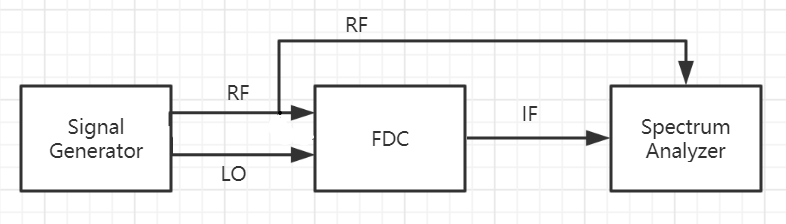
\includegraphics[width=0.8\textwidth]{img/test.png}
    \caption{\label{Fig:test}Test Circuit Diagram}
    \end{centering}
    
\end{figure}

Figure \ref{Fig:test} presents the interaction among signal generator, FDC and spectrum analyzer. RF and LO signal are expected to be generated from the signal generator and the signals are required to be transmitted to FDC with BNC connectors. The output IF of the FDC should connect to the spectrum analyzer with a BNC adapter. Besides, the spectrum of RF signal is also expected to be displayed in the same screen. As the spectrum analyzer we using may not accept two input signal at the same time, other method such as Photoshop might be considered to help to make the result more readable.

Test procedure was designed to test the response of the PCB product. 

\begin{enumerate}
 \item Give a 5.0V power supply.
 \item Give a 610MHz sine to RF input waveform and no LO input with a high frequency signal generator. Record the frequency response from IF output with a Spectrum Analyzer.
 \item Give no RF input waveform and 530MHz sine waveform to LO input with a high frequency signal generator. Record the frequency response from IF output with a Spectrum Analyzer.
 \item Give a 610MHz sine to RF input waveform and 530MHz sine waveform to LO input with a high frequency signal generator. Record the frequency response from IF output with a Spectrum Analyzer.
 \item Give a 610MHz sine to RF input waveform and 690MHz sine waveform to LO input with a high frequency signal generator. Record the frequency response from IF output with a Spectrum Analyzer.
 \item Adjust the RF input waveform and give a 530MHz sine waveform to LO input with a high frequency signal generator. Record the change of frequency response from IF output with a Spectrum Analyzer.
 \item Adjust the LO input waveform and give a 610MHz sine waveform to RF input with a high frequency signal generator. Record the change of frequency response from IF output with a Spectrum Analyzer.


\end{enumerate}





\chapter{Result and Analysis}

\section{Schematic}

\begin{figure}[htbp]     \begin{centering}
    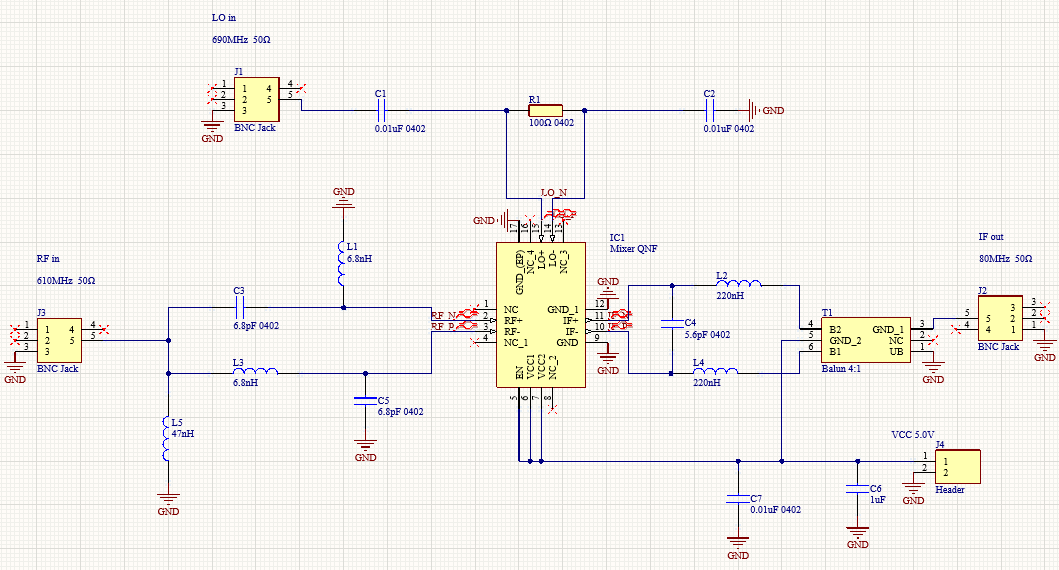
\includegraphics[width=1\textwidth]{img/sch0.png}
    \caption{\label{Fig:sch0}Schematic Result of FDC}
    \end{centering}
    
\end{figure}

Figure \ref{Fig:sch0} presents the schematic result of FDC working at frequency 610MHz-80MHz. From the perspective of interface, there are two signal input, RF and LO, one 5V power supply and a signal output of the circuit. The surrounding circuit can be divided into four parts. They are the RF part, the LO part, the power supply and IF part.

\begin{figure}[htbp]     \begin{centering}
    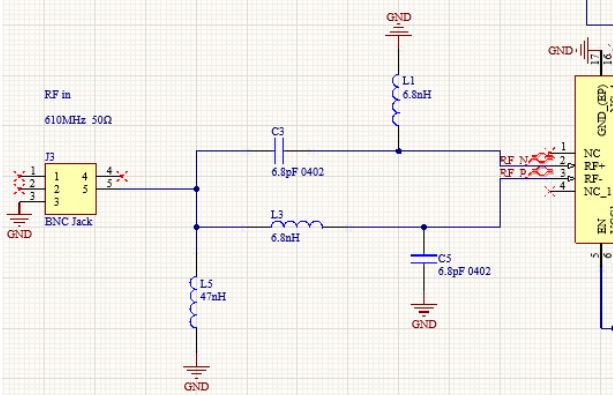
\includegraphics[width=0.5\textwidth]{img/sch0_rf.png}
    \caption{\label{Fig:sch0_rf}RF part of Schematic Result of FDC}
    \end{centering}
    
\end{figure}

\newpage

In the RF part shown in Figure \ref{Fig:sch0_rf}, signal at 610MHz is expected to be input through a 50ohms standard BNC Jack. After that, the inductor $L_{5}$ is used to short-circuit the low frequency signal. $L_{1}$ and $C_{3}$ consist a 2 orders high pass filter while $L_{3}$ and $C_{5}$ format a 2 orders LPF with the same time constant. These two filters can block the noise that at either much larger or smaller than 610MHz. Besides, these components were also designed to match the overall impedance to 50 ohms.

\begin{figure}[htbp]     \begin{centering}
    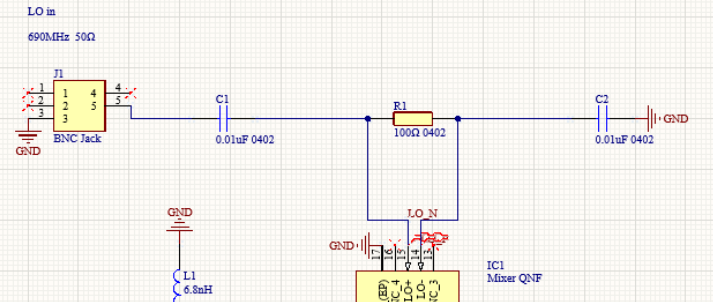
\includegraphics[width=0.5\textwidth]{img/sch0_lo.png}
    \caption{\label{Fig:sch0_lo}LO part of Schematic Result of FDC}
    \end{centering}
    
\end{figure}

In the LO part, a vibration signal is expected to be input to adjust the output frequency of the mixer. As it shown in Figure \ref{Fig:sch0_lo}, the LO signal is also expected to be input via a 50 ohms BNC jack. The input frequency can be either 530MHz or 690MHz, if the phase shift of the IF output is not considered. The two 0.01uF capacitors $C_{1}$ and $C_{2}$ are implemented to block the DC noise from the LO input signal. Besides, the resistor $R_{1}$ is used to limit the current and adjust the impedance to perfect the performance of the IC basing on practical experience.

\begin{figure}[htbp]     \begin{centering}
    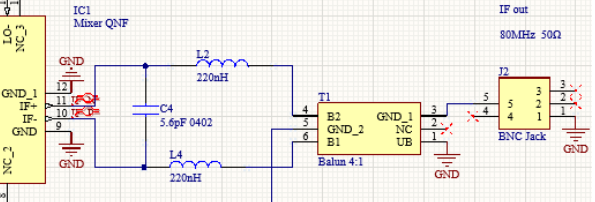
\includegraphics[width=0.5\textwidth]{img/sch0_if.png}
    \caption{\label{Fig:sch0_if}IF part of Schematic Result of FDC}
    \end{centering}
    
\end{figure}

For the IF part of the schematic shown in Figure \ref{Fig:sch0_if}, the signal is exported deferentially from the IC with around 400 ohms impedance. The capacitor $C_{4}$ is set to enhance the isolation of LO part according to the LT5512 datasheet\cite{ref:LT5512}. The components $C_{4}$, $L_{2}$ and $L_{4}$ are designed to filter the high frequency noise and match the impedance to 200ohms. After that, a 4:1 Balun transformer is used to transfer the impedance from 200ohms to 50ohms. The Balun also functions to convert the differential line to single-end line with a VCC bias on $GND_{2}$ port basing on the LT5512 datasheet\cite{ref:LT5512}. After the Balun, the output is transfer to the BNC jack to connect to other devices.

\begin{figure}[htbp]     \begin{centering}
    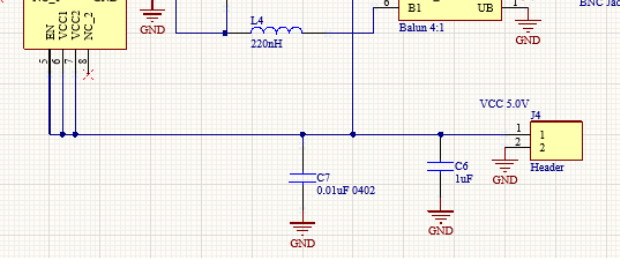
\includegraphics[width=0.5\textwidth]{img/sch0_vcc.png}
    \caption{\label{Fig:sch0_vcc}Power Supply part of Schematic Result of FDC}
    \end{centering}
    
\end{figure}

The power supply part shown in Figure \ref{Fig:sch0_vcc} is connected to a PCB header to get a 5V DC input from outside. A large capacitor $C_{6}$ is set near the header to block the low frequency noise that generated from the activities of other equipment of the electrical network. This capacitor can also gentle the transient when the power switching on and off. Approaching the IC, a small capacitor $C_{7}$ is set to further block some high frequency noise in the circuit which may be caused from the air since the power can be regarded as antenna to some extent.

Another version of schematic working at frequency 1.9GHz-170MHz was also designed but not be used as some of its components cannot be found on market. Its schematic can be found in Appendix.

\section{Bill of Materials}


\begin{table}[htbp]
\caption{Bill of Material of FDC 610MHz-80MHz}
\label{tab:bom}
\begin{center}
\resizebox{\textwidth}{!}{
\begin{tabular}{llllll}
Comment     & Description        & Designator & Footprint                       & LibRef         & Quantity \\
            &                    &            &                                 &                &          \\
0.01uF 0402 & Capacitor          & C1, C2, C7 & CAPC1005X56N                    & 0402YC103JAT2A & 3        \\
6.8pF 0402  & Capacitor          & C3, C5     & CAPC1005X56N                    & 04025A6R8CAT2A & 2        \\
5.6pF 0402  & Capacitor          & C4         & CAPC1005X56N                    & 04025A5R6CAT2A & 1        \\
1uF         & Capacitor          & C6         & CAPC1608X87N                    & 885012206052   & 1        \\
Mixer QNF   & Integrated Circuit & IC1        & QFN65P400X400X80-17N-D          & LT5512EUF\#PBF & 1        \\
BNC Jack    & Connector          & J1, J2, J3 & 5-1634506-1                     & 5-1634506-1    & 3        \\
Header      & Connector          & J4         & HDRV2W64P254\_2X1\_508X580H1118 & 22-27-2021     & 1        \\
6.8nH       & Inductor           & L1, L3     & WE-KI\_0402A30                  & 744765068A     & 2        \\
220nH       & Inductor           & L2, L4     & INDC2012X105N                   & LQM21NNR22K10D & 2        \\
47nH        & Inductor           & L5         & INDC1608X60N                    & LQP18MN47NG02D & 1        \\
100ohms 0402   & Resistor           & R1         & RESC1005X40N                    & ERA2AEB101X    & 1        \\
Balun 4:1   & Transformer        & T1         & DXP18BN5014TL                   & DXP18BN5014TL  & 1       
\end{tabular}}
\end{center}
\end{table}

Table \ref{tab:bom} displays the result if the Bill of Material. As it shown in the table, the footprint, part number and quantity of components are listed. It can be figured out that most of the passive components are in 0402 package, which may result in the rising of manufacture difficulty. 



\section{PCB Layout}


\begin{figure}[htbp]     \begin{centering}
    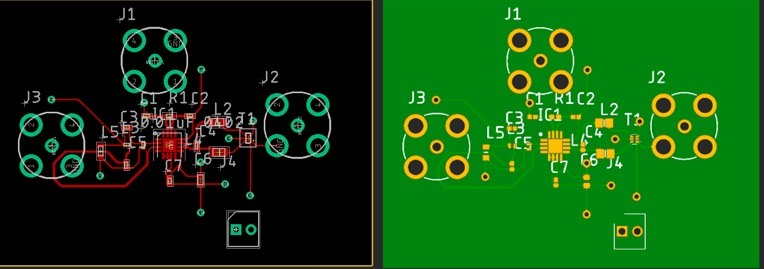
\includegraphics[width=0.7\textwidth]{img/F1.jpg}
    \caption{\label{Fig:e2} Overview of top layer}
    \end{centering}
\end{figure}

Before the PCB is put into production, the design documents must be delivered. The file submitted in *.BRD format is designed by the Autodesk Eagle v9.5.1 software. The basic layout and wiring as well as copper plating on the PCB bottom layer were completed in this design file. The component placement and the wiring on the top layer will be shown as figure \ref{Fig:e2}, and the copper plating and routing on the bottom layer will be shown as Figure \ref{Fig:e3}


\begin{figure}[htbp]     \begin{centering}
    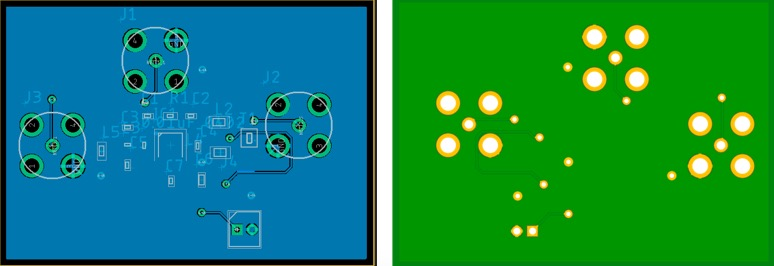
\includegraphics[width=0.7\textwidth]{img/F0.jpg}
    \caption{\label{Fig:e3} Overview of bottom layer}
    \end{centering}
\end{figure}


This design document can only be used for the manufacture of PCB samples. It is not a qualified delivery design document that can be put into production. The complete PCB design file should include schematics, * .BRD files, bills of materials, PCB design instructions, requirements for PCB design, standardization requirements and process design instructions. For further optimization, component inspection and functional inspection need to be carried out including whether the layout of high-speed signal devices is reasonable and whether the device layout meets technological requirements. The rule settings also need to be checked, and the wiring and screen printing should be further adjusted and optimized. Moreover, this design has insufficient consideration of EMC and reliability, because the focus of this task is to achieve functionality.

\section{PCB Product}

\begin{figure}[htbp]     \begin{centering}
    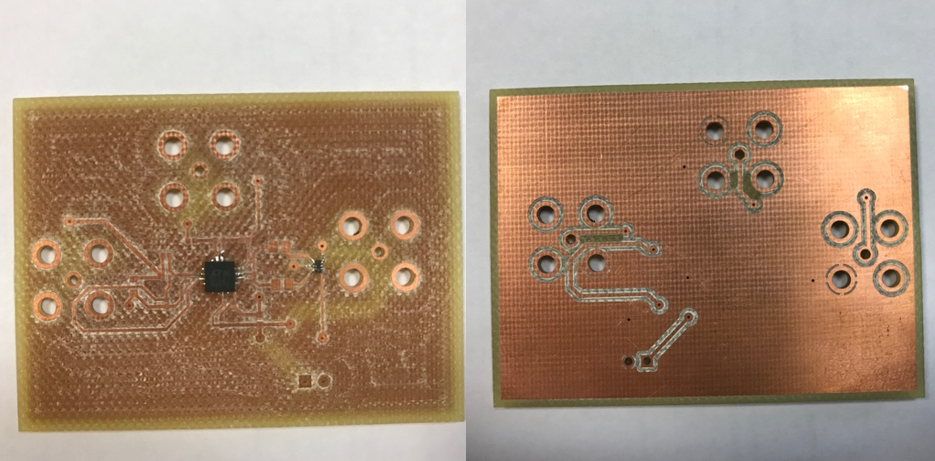
\includegraphics[width=0.7\textwidth]{img/e1.png}
    \caption{\label{Fig:e1}PCB ( Top layer and Bottom layer)}
    \end{centering}
\end{figure}


As a result, the product was not completed and the testing process could not be carried out. With the assistance of the technical department, the PCB traces, vias, and copper plating were completed shown as figure \ref{Fig:e1}. The first reason for incompleteness is the unfamiliarity with the software. The learning cycle of two design software is long, and the time for the designer to study is tight. In addition, designers did not know enough about the functions of the technical department, and the lack of information exchange with the technical department led to a delay in the submission of design documents.

\section{Test}

The test was not conducted due to incomplete PCB product.

\chapter{Discussion and Conclusions}



\section{Circuit Design}

At the first stage of circuit design, complex and reliable circuits was built. However, when more information was acknowledged, it was realized that the less work can be done due to limited time. The first version of the schematic draft consists amplifiers, op-amp, filters and was working at a high frequency of 1.9GHz. At that stage, the difficulty of components purchase, SMD manufacture, RF circuit design and PCB layout were not realized. Finally, a simple FDC schematic working at 610MHz-80MHz consists of only mixer and one LPF was designed.

Although several useless works were done due to idealism and lack of experience, an array of new skills and knowledge were obtained. Firstly, Altium Designer as a popular EDA tools was tried and learnt. The procedure of how to find and build schematic and PCB library and how to draw schematic and PCB routing were acknowledged. Secondly, the skill of looking for suitable components on supplier's website was cultivated. Thirdly, the ability to quickly locate the key information in datasheet was trained during the process of checking the datasheets of every components again and again. Fourthly, Git version control tool was introduced at the first stage of PCB layout design. The reason for using this is because when the PCB design was beginning, the version of schematic was still rolling. Since Altium Designer support Git, this method was used to help PCB designer to track the changes from the schematic. Fifthly, the design method of filters and impedance matching were acknowledged through the practical designing work. The manner of using capacitor in series with input signal to block DC noise and using different values of capacitors in parallel with the power supply line to filter the noise from the electrical network were noticed. Besides, the usage of Balun transformers was practiced converting the impedance and transform differential line to signal end line. 

\section{Components Selection}

As the most important part of components selection, the IC selection took place in last December and select LT5512 which can accept a wide range of input frequency from 10MHz to 3GHz. However, the small scale of its size resulted in significant difficulty to manufacture and PCB layout. The reason for this may be that at the first stage of the project, the requirement of the project was not perfectly understand. For example, it was confused that whether we should design a FDC that is suitable for all 300MHz-3GHz or we can select any one frequency in this range. This point was clear until the time that we begin to design with studying the datasheet. Besides, the importance of frequency selection flexibility was overrated while the significance of package size was overlooked.

Another important mistake for components selection was that the manufacture ability of university was not be detailed investigated. In fact, if it was known that the university cannot manufacture this SMD, other plan such as FPGA and hand-solder could be implemented. As the purchase of components and manufacture of PCB in department cost time, it was realized that the project timetable need to be more flexible. For example, when the PCB was manufactured, the method of testing can be considered. Besides, when selecting the components, 0402 package was preferred to follow the recommended demo in LT5512 datasheet\cite{ref:LT5512}. However, this decision finally directly gave rise to the failure of the PCB manufacture.



\section{PCB Structure Design}

In the actual work, the single-layer board is not the only choice for the design of RF circuits. However, there are several limitations in this project such as inexperienced designers, short development cycles and process limitations, so the group selected the single-layer design. In the process of RF PCB structure design, in addition to considering the impedance of the RF signal lines, issues such as heat dissipation, current, devices, electromagnetic compatibility (EMC), structure, and skin effects should also be considered. For the RF double-sided printed board, the top layer is the signal layer and the bottom layer is the ground layer.


\section{PCB Layout}
PCB layout design is one of the most important process in the entire PCB design process. With the increasement of the complexity of the PCB, the quality of the layout can directly affect the difficulty of the routing in the next step. The quality of PCB layout and design relies on the circuit design experience of the PCB designers. Therefore, as inexperienced PCB designers, it is a good approach to place components based on the datasheet of components and layout rules.

Moreover, the PCB size should be considered during the PCB layout. Once the PCB size is too large, the increase of the lead leads to an increase in impedance, a reduction in noise resistance and an increase in cost. If the PCB size is too small, the heat dissipation is not good, and adjacent wires are easily interfered. Therefore, after the PCB size is determined, and the position of the special component can be determined. Finally, according to the functional units of the circuit, all components of the circuit could be laid out.

To be specific, the distance between the high frequency components should be reduced, and it is suggested that the Distribution parameters and mutual electromagnetic interference should try to be reduced. In addition, vulnerable components should not be placed too close to each other, and input and output components should be kept as far away as possible. Furthermore, the position of each functional circuit unit based on the flow of the circuit to ensure the layout convenient for signal flow and keep the signal in the same direction as possible. Layout around the core components, components should be evenly, neatly and compactly arranged on the PCB to reduce and shorten the connections between components. For circuits operating at high frequencies, the general circuit should have components arranged in parallel as much as possible.


\section{PCB Routing}

PCB wiring design is the process with the largest workload in the entire PCB design, which directly affects the performance of the PCB board. In terms of the best signal integrity performance of the circuit board, the high speed and RF trace routing is extremely important. The impedance of traces should be kept within a narrow margin by controlling the trace width, as well as enough separation should be maintained to guard against cross-talk \cite{ref:e0}. The basic requirement of the PCB routing is to connect the circuit without short circuit and open circuit. A further requirement is the fulfilment of electrical performance, which is a specification for assessing the eligibility of a PCB. After wiring, adjust the wiring to achieve the best electrical performance. The third stage is the aesthetic requirements. The disorderly wiring will bring great inconvenience to the optimization, testing and maintenance of the later board modification, even if the electrical performance is qualified.

Equally important, there are several aspects should be improved in the process of PCB routing. The length of the RF trace should be as short as possible, and the line width should be set strictly according to the calculated value. In the routing, it is especially important to note that there should not be any sharp points in the RF routing. At the turning point of the routing, it is best to use arcs to achieve it. First, the ground wire next to the RF trace should be penetrated through the via hole and connected to the ground plane of the bottom or middle layer. Therefore, any interference signal or radiation has the shortest path to ground. However, the distance between the via and the RF signal line should not be too close, otherwise the RF signal quality will be seriously affected. During the layout of the differential pair, the two PCB lines in the differential pair should be completely the same. This means that the designer should make every effort to ensure that the PCB lines in the differential pair have exactly the same impedance, and the length of the wiring is exactly the same in practical applications.

\section{Copper Plating}
The copper of the PCB is generally connected to the ground wire to increase the area of the ground wire, which is beneficial to reduce the impedance of the ground wire and stabilize the power supply and signal transmission. Placing copper near high-frequency signal lines can greatly reduce electromagnetic radiation interference. As a result, the electromagnetic compatibility and the anti-interference ability of the PCB can be enhanced. In high-frequency circuits, the distributed capacitance of the wiring on the printed circuit board will affect the circuit to a certain extent. When the length is longer than $\frac{1}{20}$ of the corresponding wavelength of the noise frequency, an antenna effect will occur, and noise will be emitted outward through the wiring. If there is poorly grounded copper in the PCB, copper becomes a tool for transmitting noise. Therefore, in high frequency circuits, it is necessary to make holes in the wiring at a pitch smaller than $\frac{\lambda}{20}$ to make good contact with the ground plane. If the copper is treated properly, copper can not only increase the current, but also play a role in shielding interference.

\section{Impedance control}
When designing a high-speed PCB circuit, impedance matching is one of the design elements, and the impedance value has an absolute relationship with the wiring method. The characteristic impedance is related to the board layer where the PCB leads are located, the material (dielectric constant) used by the PCB, the trace width, and the distance between the leads and the plane. The characteristic impedance can be calculated using software. In high frequency signal circuits, serial impedance matching is generally used. The resistance range of the serial resistor is from 20 to 75Ω which is proportional to the signal frequency and inversely proportional to the PCB trace width and length. Altium Designer can help designer complete impedance control by incorporating PCB impedance calculations into design rules.


\section{Working Method}
During this project, students learned some management methods to improve the efficiency of group work. Specific methods are listed below.

\begin{enumerate}

\item Everyone was responsible for one type of thing. Students borrowed from the model of cooperation between various departments such as the R\&D department and the marketing department during the operation of the company.  Each student did what they did best and communicated with each other. For example, if someone has a strong ability to design circuits, then he will be responsible for the circuit design. Some people write reports quickly and well, then he will be responsible for the compilation of reports in this project. In this way, everyone was responsible for what they do best, and could maximize efficiency.
\item Write to do list. Every week, students wrote their tasks to be done on this week to the to do list. After the experiment on every Friday, checked out the things that they had completed on the to do list. Students set some realistic goals. Set over-arching, broad goals for the entire group, and then worked together to decide which goals to set for each person \cite{ref:e1}. Each task had a clear deadline and a clear point in time. For example, what to do in the morning and what to do in the afternoon on Friday. In this way, students clearly understood what they want to do each week. They had a sense of urgency, reduced ineffective communication, and achieved efficiency.
\item Used some team collaboration software. Students used GitHub, One-Drive (actually group members built a Git repository on OneDrive, and made it auto-sync with remote GitHub repository), and more. GitHub allowed students to share the latest status and progress of the group at any time. The tasks of each group were related to each other, and the exchange of information at any time allows students to better organize their time. OneDrive allows students to edit files on multiple computers together to avoid confusion during file transfer. This also allowed the team to save much time when editing a file together (such as the Supervisor weekly meeting log).
\item There was a regular meeting every week except for the experiment on Friday. Think about the content of the meeting in advance, plan a clear meeting process in advance, ask their own questions this week, and get suggestions from others in the group. Try to eliminate additional unnecessary meetings and give everyone more time to focus on the more important tasks that they are responsible for.

\end{enumerate}

But there are still many things that can be improved in the future. For example, the group had held two video conferences. When not in a face-to-face meeting, students' attention was not so concentrated, which lead to reduced efficiency and prolonged the meeting time. Next time, students can try to let one student lead the process and ask other team members to actively ask the process to make the process move faster.



\section{Applications}

The products are used in signal amplifier equipment. It can reduce the frequency of the input signal and preserve the information. The products can make a great difference in relevant equipment, including mobile phones, radar. The equipment may be used in Aeronautics and Space field. As a result, there is a promising future in the commercialization of the products

\section{Ethical Considerations}

The ethical problems are discussed in the following paragraph. Firstly, a serious-environment problem can be caused because of large-scale manufacture and sale of electronic products. Due to the complex structure of the FDC, large-scale manufacture can cost massive sources, including metal and semiconductor material. Moreover, the recycling of products also costs time and money. Improper recycling methods may release toxic substances and hurt the health of the recycle worker. As a result, obsolete products should be sent to a professional recycling company.

\section{Commercialisation and Intellectual Property}

\subsection{Commercialization}

After group discussion, two methods of commercialization are optional. Firstly, the design may be adopted by a signal equipment manufacturing company. If the group can promote the design to a manufacturing company, the design may be used in a part of the signal equipment. 

Another possible way is founding a startup company to produce electronic products. However, venture investment and professional qualifications are necessary for an electronic manufacturing company. The investment of a startup company is hard to obtain. The obtain professional qualification also cost time. It required countless future effects in the methods.


\subsection{Intellectual Property}
The products are designed by the group members. As a result, the group members have the Intellectual property of the FDC. However, group members still need to apply for the patent formally.



\section{Future Work}


There are some lessons students leaned from the projects which is helpful in the future work. First, a better communication can reduce the misunderstanding and repetition work. Then, a detailed schedule is more helpful in the actual work. As a result, in the future work, students should keep a good communication with the relevant technical partners. Moreover, a detail schedule should be finished in advance.


\section{Conclusions}
The report has presented the process of design and manufacture of a FDC. The basic circuit and the detailed PCB design are finished. The basic products of PCB have been manufactured. However, due to the tight schedule, the product is not finished and tested.

\begin{enumerate}
 \item The principle circuit of the device is designed. With a massive study of component datasheet and careful calculation in the circuit. A practical scheme was chosen, and the components are purchased.
 \item The detailed PCB design is finished with the basic PCB design principle. The group member succeed to learn how to use AD and Eagle CAD to design a PCB circuit.
 \item The PCB is manufactured.
 \end{enumerate}
 
In summary, the FDC is used to convert the high-frequency signal to a low frequency signal. It is used in signal equipment to reduce the cost of equipment. In the projects, students succeed to design and manufacture a PCB circuit. The assembling and test of products still need further work.






%-------------------------------------------- References -----------------------------------------------

\singlespace
\bibliographystyle{IEEEtran}               % References section created automatically
\bibliography{MyRefs}                      % The file MyRefs.bib contains the actual bibliography material
\addcontentsline{toc}{chapter}{References} % to add it to the table of contents


% --------------------------- This is how to declare the Appendices section ----------------------------
\newpage
\appendix
\appendixpage
\addappheadtotoc


%-------------------------------------------------------------------------------------------------------
\chapter{Extra Schematic}
%-------------------------------------------------------------------------------------------------------

This is the schematic version that working at 1.9GHz-170MHz.

\begin{figure}[htbp]     \begin{centering}
    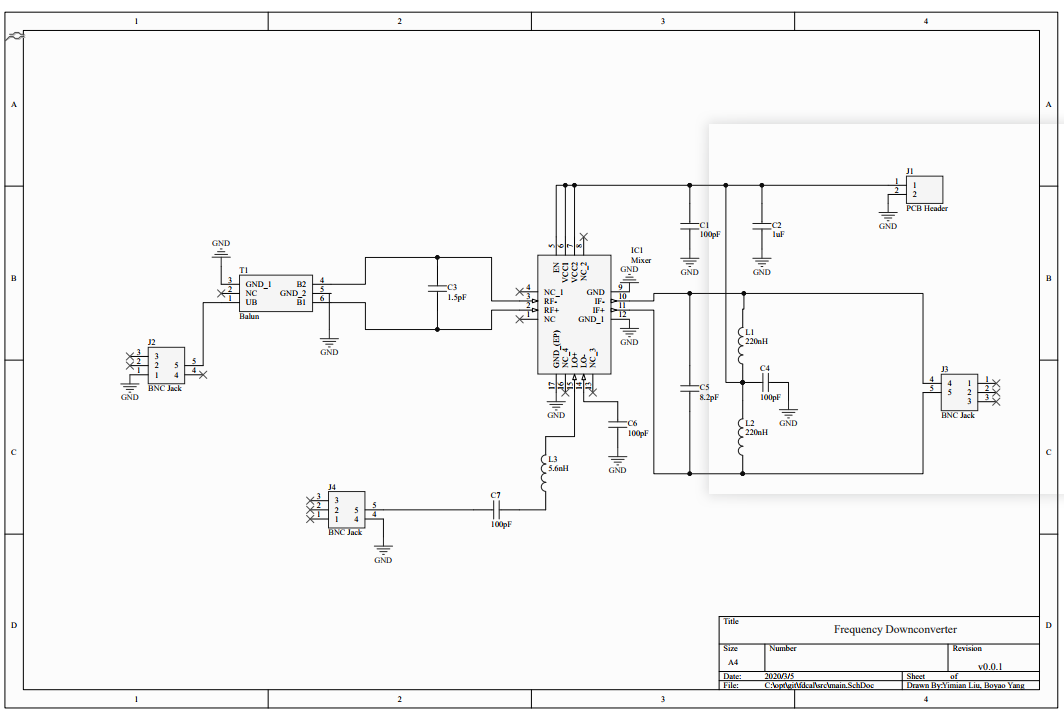
\includegraphics[width=1.2\textwidth]{img/sch1.png}
    \caption{\label{Fig:sch1}Schematic Result (1.9GHz-170MHz) of FDC}
    
    \end{centering}
    
\end{figure}

%-------------------------------------------------------------------------------------------------------
\chapter{Related Websites}
%-------------------------------------------------------------------------------------------------------
These are the related websites of this project:
\begin{enumerate}
 \item \textbf{Project Blog}: \href{https://fdc.eee.dog/}{https://fdc.eee.dog/}
 \item \textbf{Project Repository}: \href{https://github.com/IoTcat/FDC}{https://github.com/IoTcat/FDC}
 \item \textbf{Altium Repository}: \href{https://github.com/IoTcat/fdc-altium}{https://github.com/IoTcat/fdc-altium}
 \item \textbf{Report Repository}: \href{https://github.com/IoTcat/fdc-report}{https://github.com/IoTcat/fdc-report}
 \end{enumerate}

%-------------------------------------------------------------------------------------------------------
\chapter{LT5512 Datasheet}
%-------------------------------------------------------------------------------------------------------

This is the 6-10 pages of LT5512 datasheet. Full content can be found \href{https://www.analog.com/media/en/technical-documentation/data-sheets/5512fa.pdf}{here}.

\includepdf[pages=6-10]{pdf/LT5512.pdf}


\end{document}
